% CSC 586F Interim Report 1. Build with:  python report/build.py
% Measured numbers come from generated/results.tex (written by report/fill_results.py), never typed here.
\documentclass[sigconf,nonacm]{acmart}
\usepackage{booktabs}
\usepackage{algorithm}
\usepackage{algpseudocode}
\usepackage{graphicx}
\usepackage{xcolor}

\newcommand{\TBD}[1]{\textcolor{red}{\textbf{TBD\if\relax\detokenize{#1}\relax\else: #1\fi}}}
\newcommand{\code}[1]{\texttt{#1}}
\newcommand{\file}[1]{{\urlstyle{tt}\nolinkurl{#1}}}   % file paths, may break at / and .
% Generated by report/fill_results.py. Do not edit by hand.
% Source: RESULTS.md (Oct 6), notebook not run yet
\newcommand{\ResSource}{%
Oct 6 run on a Colab Tesla T4 (CuPy 14.0.1), one session. GPU times are medians of 10 runs. CPU times are the best of 3 runs (the loop ran once)}
\newcommand{\ResShort}{%
Oct 6 run}
\newcommand{\ResEnv}{%
A Colab Tesla T4 with CuPy 14.0.1. The CPU model of that session was not recorded.}
\newcommand{\GatherMsMedium}{%
1.52}
\newcommand{\GatherMsLarge}{%
4.90}
\newcommand{\ScatterMsMedium}{%
25.5}
\newcommand{\ScatterMsLarge}{%
246.5}
\newcommand{\ScipyMsMedium}{%
989}
\newcommand{\ScipyMsLarge}{%
4,389}
\newcommand{\LoopMsMedium}{%
13,935}
\newcommand{\AblationMedium}{%
16.8}
\newcommand{\AblationLarge}{%
50.3}
\newcommand{\VsScipyMedium}{%
652}
\newcommand{\VsScipyLarge}{%
896}
\newcommand{\VsLoopMedium}{%
9,186}
\newcommand{\VsCppMedium}{%
\TBD{run notebook}}
\newcommand{\VsCppLarge}{%
\TBD{run notebook}}
\newcommand{\FullSizeVerdict}{%
On October 6, on the GPU, both kernels matched the CPU reference on the medium and large instances. The largest relative errors were 4.9e-7 and 4.8e-7 for scatter and 9.9e-7 and 1.2e-6 for gather.}
\newcommand{\ResCaveat}{%
The October 6 numbers come from one session, with medians of 10 runs on the GPU but the best of 3 runs, or a single run for the loop, on the CPU.}
\newcommand{\GatherGBps}{%
125}
\newcommand{\KernelRows}{%
medium & 13,935 & 989 & \TBD{} & 25.5 & \textbf{1.52} \\
large & not run & 4,389 & \TBD{} & 246.5 & \textbf{4.90} \\}
\newcommand{\SpeedupRows}{%
gather vs scatter (ablation) & not run & 16.8$\times$ & 50.3$\times$ \\
gather vs CPU scipy product & not run & 652$\times$ & 896$\times$ \\
gather vs CPU loop & not run & 9,186$\times$ & not run \\
gather vs CPU C++ (Alg. 1) & \TBD{} & \TBD{} & \TBD{} \\}
\newcommand{\EndToEndVerdict}{%
\TBD{run notebook}}
\newcommand{\ProfileVerdict}{%
\TBD{run notebook}}
\newcommand{\CorrectnessVerdict}{%
\TBD{run notebook}}
\newcommand{\NotebookStatus}{%
\TBD{The notebook has not been run yet. Tables~\ref{tab:correct}, \ref{tab:e2e} and \ref{tab:profile} are placeholders until it has.}}
\newcommand{\InstanceRows}{%
small & 2,000 $\times$ 20,000 & 3.2 M & 61.3 M & 19.1 & 1.92 M \\
medium & 4,000 $\times$ 50,000 & 16.0 M & 311.9 M & 19.5 & 3.84 M \\
large & 8,000 $\times$ 120,000 & 76.8 M & 1.51 G & 19.7 & 7.68 M \\}
\newcommand{\TermsMedium}{%
311.9 M}
\newcommand{\NnzMedium}{%
16.0 M}
\newcommand{\SelPerCellMedium}{%
19.5}
\newcommand{\GatherAddsMedium}{%
512.0 M}
\newcommand{\WorkRatioMedium}{%
1.64}
\newcommand{\WorkRatioLarge}{%
1.62}
\newcommand{\ShuffleAddsMedium}{%
614.4 M}
\newcommand{\SegLenMedium}{%
133}
\newcommand{\SegLenLarge}{%
320}
\newcommand{\ThreadsMedium}{%
3,840,000}
\newcommand{\ThreadsLarge}{%
7,680,000}
\newcommand{\ScatterThreads}{%
230,400}
\newcommand{\CorrectnessRows}{%
one warp & \TBD{} & \TBD{} \\
one block, several warps & \TBD{} & \TBD{} \\
several blocks & \TBD{} & \TBD{} \\
\midrule
integer data, bit-exact & \TBD{} & \TBD{} \\
worst rel. error (float data) & \TBD{} & \TBD{} \\}
\newcommand{\EndToEndRows}{%
scatter & \TBD{} & \TBD{} & \TBD{} & \TBD{} & \TBD{} \\
gather & \TBD{} & \TBD{} & \TBD{} & \TBD{} & \TBD{} \\
\midrule
CPU C++ (Alg. 1) & & & & & \TBD{} \\
CPU scipy product & & & & & \TBD{} \\}
\newcommand{\ProfileRows}{%
GPU utilisation (nvidia-smi) & \TBD{} & \TBD{} \\
memory utilisation (nvidia-smi) & \TBD{} & \TBD{} \\
registers per thread (ptxas) & \TBD{} & \TBD{} \\
stack frame, bytes (ptxas) & \TBD{} & \TBD{} \\
achieved occupancy (Nsight) & \TBD{} & \TBD{} \\}


\settopmatter{printfolios=true}
\setlength{\textfloatsep}{8pt plus 2pt minus 2pt}
\setlength{\dbltextfloatsep}{8pt plus 2pt minus 2pt}
\emergencystretch=1.5em
\raggedbottom

\begin{document}

\title{Pseudo-Bulk RNA-seq Generation on the GPU}
\subtitle{CSC 586F Interim Report 1, Group 19}
\author{Jason Thomo}
\affiliation{%
  \institution{University of Victoria}
  \city{Victoria}
  \state{BC}
  \country{Canada}}
\email{jthomo@uvic.ca}

\begin{abstract}
A pseudo-bulk RNA-seq profile is the sum of the expression of a chosen set of single cells.
Generating $P$ of them is the sparse product $PB = S X^{\top}$ of a 0/1 selection matrix and the
gene-by-cell expression matrix. This report gives a sequential reference, two CUDA kernels for the
product, and a first set of experiments. The first kernel scatters every nonzero into the output
with atomic adds. The second uses a redesigned data layout so that one warp gathers one output
segment in registers, with no atomics. On synthetic data with the structure of the real data, on a
Colab T4,
the gather kernel takes \GatherMsMedium{} ms and \GatherMsLarge{} ms on inputs of 16.0 and 76.8
million nonzeros, which is \AblationMedium{}$\times$ and \AblationLarge{}$\times$ faster than the
scatter kernel (\ResShort{}). Code: \TBD{git repository URL}.
\end{abstract}

\maketitle

\section{Introduction}

Single-cell RNA sequencing measures gene expression one cell at a time and gives a sparse matrix
with one row per gene and one column per cell. Bulk RNA sequencing measures a whole tissue sample at
once. A \emph{pseudo-bulk} imitates a bulk sample by summing the expression of a set of single
cells. Because the type of every cell is known, the cell-type fractions of a pseudo-bulk are known
exactly, which makes pseudo-bulks a standard way to build test data for cell-type deconvolution
methods~\cite{avilacobos2020}.

I chose this problem because it is a step in my own research pipeline. There, an R script builds 900
pseudo-bulks from a matrix of 14,378 genes by 241,924 cells from 30 donors. Each pseudo-bulk sums a
random subset of the cells of a single donor, so no pseudo-bulk mixes donors. On the Narval cluster
that script takes about 17 minutes and 48 GB of memory. That figure was measured outside this
project and is not reproduced here. The instructor approved the topic on October 6.

The computation is a sparse matrix product with a dense result. It has a lot of data and simple
loops, which is the shape of problem a GPU is good at, and it belongs to the sparse matrix
multiplication family. The interesting part is not the arithmetic, which is only additions, but how
the data is laid out and which thread owns which output.

This report covers the first milestone. It contains (1) a formal statement of the problem and a
sequential algorithm, (2) three CPU references, (3) two CUDA kernels of my own, a scatter kernel and
a gather kernel built on a new data layout, (4) a PRAM analysis of both, and (5) an experiment
harness with first results. \textbf{All results are on synthetic data.} The synthetic data has the
structure of the real data (30 donors, 30 pseudo-bulks per donor, sparse CPM columns) but is smaller,
at most 8,000 genes by 120,000 cells. The real data sits on a cluster and has not been run yet. That
is the first item of future work.

\section{Background}

\paragraph{Inputs.} There are $G$ genes, $C$ cells and $D$ donors. Each cell belongs to exactly one
donor. $X$ is a sparse $G \times C$ matrix with $N$ nonzeros, and $X[g,c]$ is the expression of gene
$g$ in cell $c$ in counts per million (CPM), so each column sums to $10^6$. Each donor gets $K$
pseudo-bulks, so there are $P = DK$ in total. The selection matrix $S$ is a 0/1 matrix of size
$P \times C$, and $S[p,c] = 1$ means cell $c$ is in pseudo-bulk $p$. Row $p = dK + k$ only selects
cells of donor $d$. $S$ is drawn once on the host: for each pseudo-bulk a ratio $r$ is drawn
uniformly from $[0.3, 1]$ and $\lfloor r\,n_d \rfloor$ of the donor's $n_d$ cells are chosen without
replacement. $S$ is an input, so every implementation is given the same $S$ and their outputs can be
compared entry by entry.

\paragraph{Output.} A dense $P \times G$ matrix
\begin{equation}
PB = S X^{\top}, \qquad PB[p,g] = \sum_{c\,:\,S[p,c]=1} X[g,c],
\label{eq:pb}
\end{equation}
followed by a scaling of each row so it sums to $10^6$ again. The real problem has $G = 14{,}378$,
$C = 241{,}924$, $D = 30$ and $K = 30$, so $P = 900$.

\paragraph{Size of the sum.} Let $n_c$ be the number of nonzeros of cell $c$ and $t_c$ the number of
pseudo-bulks that selected it, with $0 \le t_c \le K$. Equation~\ref{eq:pb} has
$F = \sum_c t_c\,n_c$ terms in total. $F$ is the amount of arithmetic the problem contains.

\begin{algorithm}[t]
\caption{Sequential pseudo-bulk generation. $X$ is stored by cell (CSC), $S$ by pseudo-bulk (CSR).}
\label{alg:seq}
\begin{algorithmic}[1]
\For{$p \gets 0$ \textbf{to} $P-1$}
  \State $PB[p, \cdot] \gets 0$
  \For{each cell $c$ with $S[p,c] = 1$}
    \For{each nonzero $(g, v)$ of column $c$ of $X$}
      \State $PB[p,g] \gets PB[p,g] + v$
    \EndFor
  \EndFor
  \State $PB[p, \cdot] \gets 10^6 \cdot PB[p, \cdot] \,/\, \sum_g PB[p,g]$
\EndFor
\end{algorithmic}
\end{algorithm}

\paragraph{Sequential algorithm.} Algorithm~\ref{alg:seq} does one addition per term, plus a
constant amount of work per output entry, so it runs in $\Theta(F + PG)$ time. It is the row-by-row
sparse product with a dense accumulator described by Gustavson~\cite{gustavson1978}. I use it as the
sequential baseline $T_{seq}$ in the analysis.

\paragraph{CPU references.} The repository has three, all single-threaded. (1) \code{compute\_loop}
is a Python port of the R script. It multiplies all of $X$ by an indicator vector once per
pseudo-bulk, which costs $\Theta(PN)$ and is slower than Algorithm~\ref{alg:seq}. (2)
\code{compute\_batched} computes $S X^{\top}$ with one SciPy sparse product~\cite{scipy2020}. (3)
\file{seq_ref.cpp} is Algorithm~\ref{alg:seq} in C++, compiled with \code{-O3}. Unit tests check
that the three agree with each other and with a dense computation, that every row sums to $10^6$,
and that no pseudo-bulk contains cells of two donors.

\section{Methods}

\subsection{Where the parallelism is}

Unrolling Algorithm~\ref{alg:seq} gives $F$ terms. Term $(p, c, g)$ adds $X[g,c]$ into $PB[p,g]$.
Terms for different output entries do not interact. Terms for the same entry form a sum, which can be
grouped in any order. So the problem is $PG$ independent reductions, and the same instruction, an
add, is applied to all the data. That is data-level parallelism. The design question is how to give
threads to terms. Giving each thread a piece of the \emph{input} and letting it write wherever its
terms go is a scatter. Giving each group of threads a piece of the \emph{output} and letting it
collect its terms is a gather. I implemented both (Figure~\ref{fig:par}).

\begin{figure*}[t]
\centering
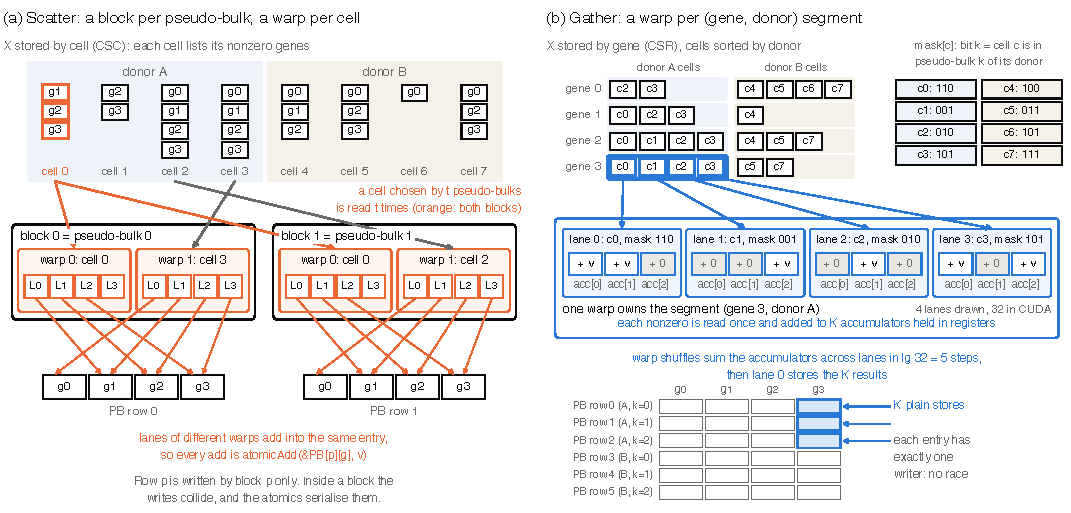
\includegraphics[width=\textwidth]{figures/fig_parallelism.pdf}
\caption{How the two kernels expose parallelism, drawn from a real toy instance (4 genes, 8 cells, 2
donors, $K = 3$, warps drawn with 4 lanes). (a) Scatter gives each pseudo-bulk a block and each
selected cell a warp. Lanes add the cell's nonzeros into the output row with atomics. (b) Gather
gives each (gene, donor) segment of the reordered matrix one warp. Lanes add each nonzero into $K$
register accumulators chosen by the cell's bit mask, then the warp combines them and writes $K$
outputs that no other warp touches.}
\label{fig:par}
\end{figure*}

\subsection{Version 1: the scatter kernel}

\code{pb\_scatter} keeps the data as Algorithm~\ref{alg:seq} has it. The grid has one thread block
per pseudo-bulk, 256 threads each. Inside block $p$, warp $w$ takes the selected cells
$w, w+8, w+16, \dots$ of the pseudo-bulk, and lane $l$ of the warp takes nonzeros $l, l+32, \dots$ of
the warp's current cell and adds each one into row $p$ of the output.

Two levels of parallelism are used. Blocks are a thread-level strategy: each block does one whole
pseudo-bulk and never talks to another block. Inside a warp the lanes are data-parallel: one
instruction, 32 nonzeros.

\paragraph{Race conditions.} Block $p$ is the only writer of row $p$, so blocks cannot race. Inside
a block, two lanes race whenever their nonzeros have the same gene, which is common. Every add is
therefore an \code{atomicAdd}~\cite{cudaguide}, which makes the read, add and write one indivisible step. The order
in which atomics commit is not fixed, and floating-point addition is not associative, so the last
bits of the result can change from run to run.

\paragraph{Cost in the memory model.} A cell selected by $t_c$ pseudo-bulks is read from global
memory $t_c$ times, once per block. The reads of one cell are coalesced~\cite{cheng2014}, because
consecutive lanes read consecutive elements. The writes are not: they go to whatever genes the cell expresses, and
each one is an atomic that is serialised at L2. The kernel does $F$ nonzero reads and $F$ atomic adds.

\subsection{Version 2: a new layout and the gather kernel}

The redesign rests on one fact about the problem: a cell belongs to one donor, so only that donor's
$K$ pseudo-bulks can ever use it. Three changes follow. All three are made once, on the host, by the
function \code{build\_donor\_layout}.
\begin{enumerate}
\item Cells are sorted by donor.
\item $X$ is stored by gene (CSR) instead of by cell. With the cells sorted, the nonzeros of gene $g$
that belong to donor $d$ are one contiguous \emph{segment}, and \code{seg\_ptr}$[gD+d]$ marks where
it starts.
\item $S$ is replaced by one 32-bit mask per cell. Bit $k$ of \code{mask}$[c]$ is set when cell $c$
is in pseudo-bulk $k$ of its donor. This needs $K \le 32$.
\end{enumerate}

\code{pb\_gather} (Figure~\ref{fig:code}) gives one warp to each (gene, donor) segment. Blocks have
128 threads, so a block holds four segments, but the block has no role beyond packaging because
warps never communicate. Lane $l$ reads nonzeros
$l, l+32, \dots$ of the segment. For each one it loads the value $v$ and the cell's mask $m$, and for
every $k$ it adds $v$ to \code{acc[k]} if bit $k$ of $m$ is set and adds $0$ otherwise. The select is
branch-free, so the lanes do not diverge. When the segment is used up, a
\code{\_\_shfl\_down\_sync} reduction~\cite{cudaguide} adds the 32 lanes' copies of each accumulator in
$\lg 32 = 5$ steps, and lane 0 stores the $K$ sums to $PB[dK+k,\,g]$. The thread assignment is the
one Bell and Garland use in their CSR vector kernel for sparse matrix-vector
products~\cite{bell2008}, one warp per row with a warp-wide reduction. What is specific here is the
split of each row into donor segments and the bit mask, which lets one pass over a nonzero serve all
$K$ pseudo-bulks at once.

\begin{figure}[t]
\footnotesize
\begin{verbatim}
// one warp = one (gene g, donor d) segment, "pair"
float acc[32] = {0};
for (int i = seg_ptr[pair] + lane;
         i < seg_ptr[pair + 1]; i += 32) {
    const float v = val[i];
    const unsigned m = mask[col[i]];
    for (int k = 0; k < 32; ++k)        // unrolled
        acc[k] += ((m >> k) & 1u) ? v : 0.f;
}
for (int k = 0; k < 32; ++k) {          // unrolled
    float s = acc[k];
    for (int o = 16; o > 0; o >>= 1)
        s += __shfl_down_sync(0xffffffffu, s, o);
    if (lane == 0 && k < K)
        PB[((size_t)d * K + k) * n_genes + g] = s;
}
\end{verbatim}
\caption{The body of \code{pb\_gather}, lightly abridged from \file{pbulk/kernels.cu}.}
\label{fig:code}
\end{figure}

\paragraph{Why there are no race conditions.} (1) Every input array is read-only. (2) The
accumulators are local variables of a thread, so no other thread can write them. (3) The shuffles are
executed by all 32 lanes of the warp together. The only branch before them is the early return for
warps past the last segment, and that test has the same outcome for the whole warp. (4) The output
address is a one-to-one function of $(g, d, k)$, and only lane 0 of the warp that owns $(g, d)$
writes it. So every output entry has exactly one writer and no two threads ever write the same
address. The kernel needs no atomics, no \code{\_\_syncthreads()} and no shared memory. The additions
also happen in a fixed order, so the result is the same on every run.

\paragraph{Cost in the memory model.} Each nonzero is read once, so the kernel does $N$ nonzero
reads instead of $F$. On the medium instance of Section~\ref{sec:exp} that is \NnzMedium{} against
\TermsMedium{}, a factor of \SelPerCellMedium{}. The reads of \code{val} and \code{col} are
coalesced. The reads of \code{mask} are scattered, but sorting cells by donor confines them to one
donor's part of an array of only $4C$ bytes. All $F$ atomics are gone and are replaced by $PG$ plain
stores.

\paragraph{Why registers and not shared memory.} The lecture on shared memory gives two conditions
for it to pay off: the data is reused, and the per-thread state is too big for
registers~\cite{csc586f}. Neither holds here. Each nonzero is used once, and a thread's state is $K$
running sums. This is the reduction case from the same lecture, where the right home for the data is
registers and the exchange between lanes is a warp shuffle. Whether the compiler really keeps the 32
accumulators in registers is checked from the register and stack report of \code{ptxas}
(Table~\ref{tab:profile}).

\subsection{PRAM analysis}

I use the CRCW arbitrary PRAM of the course~\cite{casanova2008,csc586f}, where concurrent writes to
one cell must be atomics and atomics on one cell are serialised. Table~\ref{tab:pram} compares the
sequential algorithm with idealised versions of both kernels, one processing unit (PU) per unit of
work. $h_{max}$ is the largest number of terms that land in one output entry, and $L_{max}$ is the
longest segment. The row normalisation adds a $\Theta(\lg G)$ reduction per row to both parallel
times and is left out of the table.

\begin{table}[t]
\caption{Work and time on a CRCW arbitrary PRAM.}
\label{tab:pram}
\small
\begin{tabular}{@{}lccc@{}}
\toprule
 & Sequential & Scatter & Gather \\
\midrule
PUs & 1 & $F$ & $KN$ \\
Work & $\Theta(F + PG)$ & $\Theta(F + PG)$ & $\Theta(KN + PG)$ \\
Time & $\Theta(F + PG)$ & $\Theta(h_{max})$ & $\Theta(\lg L_{max})$ \\
Atomics & 0 & $F$ & 0 \\
\bottomrule
\end{tabular}
\end{table}

\paragraph{Scatter.} It does exactly the additions of Algorithm~\ref{alg:seq}, so its work equals
the sequential work. Its time is poor: all terms of one output entry are atomics on one address, so
they run one after another, and $h_{max}$ can be as large as the number of cells in a pseudo-bulk.

\paragraph{Gather.} With one PU per nonzero and accumulator, the selects take one step and each
output entry is a reduction tree over its segment, so the time is $\Theta(\lg L_{max})$. The work is
$\Theta(KN + PG)$, because every nonzero is offered to all $K$ accumulators whether its cell was
selected or not. Is that more than the sequential $\Theta(F + PG)$? Here it is not. Each pseudo-bulk
takes at least 30\% of its donor's cells and 65\% on average, so $F \approx 0.65\,KN$ and the two
are within a constant. On the medium instance the kernel does \GatherAddsMedium{} select-adds
($32N$, the kernel always carries 32 accumulators) against $F = $ \TermsMedium{} sequential adds, a
ratio of \WorkRatioMedium{}. So the gather strategy is work-efficient for this problem: run on one
thread it takes the same asymptotic time as Algorithm~\ref{alg:seq}. This depends on the sampling
rule. If pseudo-bulks took a tiny fraction of the cells, $F$ would be far below $KN$ and scatter,
whose work is always $F$, would be the work-efficient choice.

\paragraph{From the PRAM to the kernel.} The kernel does not launch $KN$ threads. It uses Brent's
theorem~\cite{brent1974}: each segment's PUs are folded onto the 32 lanes of one warp, and a lane
loops over its share. A segment of length $L$ then takes $\lceil L/32 \rceil$ loop steps and 5
shuffle steps per accumulator. The reduction is not free. All 32 lanes execute all 5 steps for all
32 accumulators, which is 5,120 adds per segment where a tree needs 992. On the medium instance that
is \ShuffleAddsMedium{} adds, more than the main loop. It is still $\Theta(PG)$ work, but it is the
first overhead I want to measure.

\paragraph{Thousands of threads.} The gather kernel launches $32\,GD$ threads: \ThreadsMedium{} on
the medium instance, \ThreadsLarge{} on the large one and 13,802,880 at the real shape. The scatter
kernel launches $256\,P = $ \ScatterThreads{} for every instance. A T4 has 2,560 CUDA
cores~\cite{t4datasheet}, and the rule from the threading lecture is that a GPU needs about 16
threads in flight per core, 40,960 here, before it is used well~\cite{csc586f}. Both kernels are far
past that, and warps never wait for each other, so extra blocks simply queue. The thread count of
gather grows with $GD$. More cells per donor make segments longer, not more numerous (about
\SegLenMedium{} nonzeros per segment on the medium instance and \SegLenLarge{} on the large one).
The lecture on multi-warp execution calls a strided loop over the input a sign that parallelism was
left unexposed~\cite{csc586f}. That is fair here, and splitting long segments across the warps of a
block is future work. It costs little today because the device is already oversubscribed.

\section{Experiments}
\label{sec:exp}

\subsection{Harness and setup}

Everything runs from one command, \code{python -m bench.ir1}, which the Colab notebook
\file{notebooks/ir1_colab.ipynb} calls on a T4 runtime. It writes one JSON file. A second command,
\code{python} \file{report/build.py}, turns that file into the tables and Figure~\ref{fig:time} of this
report, so no measured number is typed by hand. The kernels are compiled from
\file{pbulk/kernels.cu} with CuPy's \code{RawModule}~\cite{okuta2017}. Kernel times are taken with CUDA events after
warm-up runs, with all inputs already on the device. They include the row normalisation, which CuPy
does with a row sum and an element-wise multiply, and for scatter the zeroing of the output.

\paragraph{Data.} The generator gives every cell exactly $0.08\,G$ nonzeros at random genes with
log-normal values scaled to CPM, and assigns cells to 30 donors at random. $K = 30$ throughout
(Table~\ref{tab:inst}). This copies the structure of the real data: donors, pseudo-bulks per donor
and CPM columns. It does not copy the spread of nonzeros per cell or of cells per donor, which are
even here and uneven in real data, and the instances are smaller than the real matrix.

\begin{table}[t]
\caption{Synthetic instances. $F/N$ is the average number of pseudo-bulks that use a cell. Counted
from the instances, not measured.}
\label{tab:inst}
\small
\begin{tabular}{@{}lrrrrr@{}}
\toprule
 & genes $\times$ cells & $N$ & $F$ & $F/N$ & threads \\
\midrule
\InstanceRows
\bottomrule
\end{tabular}
\end{table}

\paragraph{Environment.} \ResEnv{} Baselines: the CPU loop, the SciPy product and the C++
Algorithm~\ref{alg:seq}, each on one thread. \NotebookStatus

\subsection{Correctness}

The rule is the same $S$ in, the same $PB$ out. There are four layers of evidence.

(1) \emph{Reference.} The three CPU references agree with each other and with a dense computation in
the unit tests.

(2) \emph{Kernel source on the CPU.} A small emulator compiles \file{kernels.cu} as C++ and runs the
32 lanes of each warp as coroutines that meet at every shuffle. It executes the real kernel code,
not a model of it. It cannot show races between warps, which Section 3 rules out by argument.

(3) \emph{A sweep of instances.} Eleven hand-picked instances and a set of random ones cover a
launch of one warp, one block of several warps and several blocks for each kernel, plus the edge
cases: $K = 1$, $K = 32$, every cell selected, empty segments, segment lengths that are and are not
multiples of 32, a donor with a single cell, and a partly filled last block. Each instance is run
twice. With real-valued data the output is compared with a float64 reference. With small integer
data every float32 sum is exact in any order, so the output must match bit for bit. The whole sweep
passes on the emulator. \CorrectnessVerdict{} Table~\ref{tab:correct} gives the GPU result.

(4) \emph{Full-size runs.} \FullSizeVerdict{} These launches need thousands of blocks.

\begin{table}[t]
\caption{Instances passed on the GPU, by the part of the thread hierarchy the launch needs.}
\label{tab:correct}
\small
\begin{tabular}{@{}lrr@{}}
\toprule
Launch needs & scatter & gather \\
\midrule
\CorrectnessRows
\bottomrule
\end{tabular}
\end{table}

\paragraph{Precision.} The GPU sums in float32. The SciPy reference also sums in float32, because it
keeps the input type, and only normalises in float64. Relative differences near $10^{-6}$ are
rounding from a different order of additions, not errors. The sweep in layer 3 uses a true float64
reference.

\subsection{Kernel time and the layout ablation}

\begin{figure}[t]
\centering
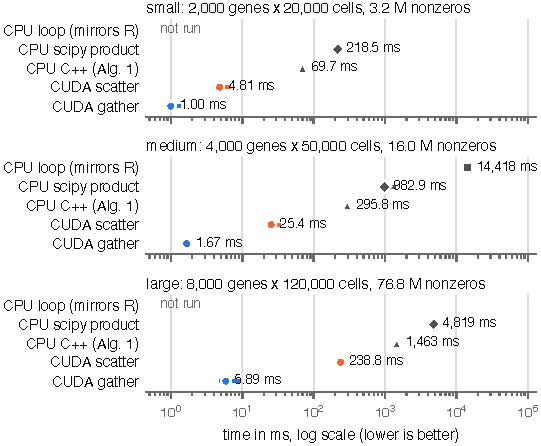
\includegraphics[width=\columnwidth]{figures/fig_timing.pdf}
\caption{Time per implementation on synthetic data, without transfers. \ResShort{}.}
\label{fig:time}
\end{figure}

\begin{table}[t]
\caption{Time in ms on synthetic data. GPU times exclude transfers and kernel compilation. Source:
\ResSource.}
\label{tab:kernel}
\small
\begin{tabular}{@{}lrrrrr@{}}
\toprule
 & CPU loop & SciPy & C++ & scatter & gather \\
\midrule
\KernelRows
\bottomrule
\end{tabular}
\end{table}

\begin{table}[t]
\caption{Speedup of the gather kernel, from Table~\ref{tab:kernel}.}
\label{tab:speed}
\small
\begin{tabular}{@{}lrrr@{}}
\toprule
 & small & medium & large \\
\midrule
\SpeedupRows
\bottomrule
\end{tabular}
\end{table}

Table~\ref{tab:kernel} and Figure~\ref{fig:time} give the times and Table~\ref{tab:speed} the
ratios. With transfers excluded, the gather kernel is \VsScipyMedium{}$\times$ and
\VsScipyLarge{}$\times$ faster than the single-threaded SciPy product on the medium and large
instances, and \VsLoopMedium{}$\times$ faster than the loop that mirrors the R script on the medium
one. Against the C++ baseline the factors are \VsCppMedium{} and \VsCppLarge{}.

Scatter against gather is the ablation of the memory layout. Both kernels compute the same sums on
the same device. They differ in the layout of $X$ and $S$ and in where the partial sums live. The
redesign makes the kernel \AblationMedium{}$\times$ faster on the medium instance and
\AblationLarge{}$\times$ faster on the large one. The operation counts explain the direction: scatter
reads each nonzero $F/N \approx 19.5$ times and issues $F$ atomics, gather reads it once and issues
none. I have not profiled why the gap widens with size, so I do not claim a cause yet. The ablation
changes the layout and the removal of atomics together. Separating the two needs a third kernel and
is future work.

As a rough utilisation check, the gather kernel streams the 8 bytes of \code{col} and \code{val} per
nonzero of the large instance at \GatherGBps{} GB/s or more, counting the whole measured time. The T4
datasheet gives 300 GB/s of memory bandwidth~\cite{t4datasheet}.

\paragraph{Caveats.} The data is synthetic. The SciPy and loop baselines are Python on Colab's CPU,
not tuned C++, and the 17 minute R figure was not measured here. \ResCaveat

\subsection{End to end, with transfers}

The kernel time hides the host side. On October 6 the upload plus the layout build took 0.69 s and
3.2 s for the two sizes, far more than the kernels and of the same order as the SciPy product. The
layout build is NumPy code on one CPU thread and is the real bottleneck of the gather path.
Table~\ref{tab:e2e} splits the wall time of each path on the medium instance into host preparation
(a type conversion for scatter, the layout build for gather), the host-to-device copy, launch plus
kernel, and the copy of the result back. \EndToEndVerdict

\begin{table}[t]
\caption{End-to-end wall time in ms on the medium instance, median of 5 runs after one warm-up.
Pageable host memory. Kernel compilation excluded.}
\label{tab:e2e}
\small
\begin{tabular}{@{}lrrrrr@{}}
\toprule
 & host prep & H2D & kernel & D2H & total \\
\midrule
\EndToEndRows
\bottomrule
\end{tabular}
\end{table}

\subsection{Device utilisation}

Table~\ref{tab:profile} collects what can be measured on Colab. \code{nvidia-smi} is sampled every
100 ms while a kernel runs in a loop. Its GPU utilisation is the share of time a kernel was running
and its memory utilisation is the share of time device memory was being read or written. Both are
coarse: they say the device was busy, not how well each SM was used. \code{ptxas} reports the
registers per thread and the stack frame of each kernel, which shows whether the accumulators stayed
in registers. The notebook also tries Nsight Compute for occupancy and throughput counters, which
Colab may not permit. \ProfileVerdict

\begin{table}[t]
\caption{Device utilisation per kernel.}
\label{tab:profile}
\small
\begin{tabular}{@{}lrr@{}}
\toprule
 & scatter & gather \\
\midrule
\ProfileRows
\bottomrule
\end{tabular}
\end{table}

\section{Future work}

For the next milestone, in this order.
\begin{enumerate}
\item \textbf{Real data.} Export the real matrix from the cluster with \file{scripts/export_sc.R}
and rerun everything. Real cells differ in nonzeros and donors differ in cell count, so segment
lengths will be uneven and the numbers will move. R's random generator cannot be reproduced in
Python, so the comparison with the R output will be statistical.
\item \textbf{Profile.} Use Nsight Compute to get occupancy and memory throughput, to find why the
gap between the kernels grows with size, and to measure the cost of the shuffle reduction.
\item \textbf{Build the layout on the GPU.} Grouping nonzeros by (gene, donor) is a counting sort on
a small key, which the course has just covered. It would remove the host bottleneck of
Table~\ref{tab:e2e}. Pinned host memory is a smaller step in the same direction.
\item \textbf{Long segments.} Split a long segment across the warps of a block and combine their
partial sums in shared memory, so that thread count follows $N$ and not only $GD$.
\item \textbf{A finer ablation.} A kernel with the new layout but atomic adds would separate the
gain of the layout from the gain of dropping atomics.
\item \textbf{Limits.} Support $K > 32$ with more than one mask word, and trim the reduction to $K$
accumulators. Whether a dense formulation could use tensor cores is an open question for the final
report.
\end{enumerate}

\bibliographystyle{ACM-Reference-Format}
\bibliography{refs}

\end{document}
